\documentclass{article}
\usepackage{amsmath}
\usepackage{amssymb}
\usepackage{graphicx}
\usepackage{hyperref}
\usepackage[version=4]{mhchem}


\begin{document}
In right \(\triangle A B C, A D\) is the height and \(P\) is the midpoint of \(A D\).\\
Connect \(B P\) and extend it to meet \(A C\) at \(E\). Suppose that \(A C: A B=k\), what is the value of \(A E / E C\) ?\\
(A) \(\frac{1}{1+k^{2}}\)\\
(B) \(\frac{1}{1+k}\)\\
(C) \(\frac{2}{1+k^{2}}\)\\
(D) \(1+k\)\\
(E) \(\frac{2}{1+k}\)\\
\centering
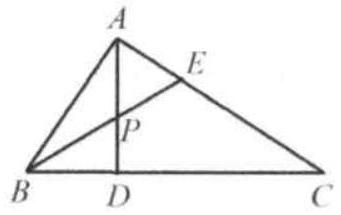
\includegraphics[width=\textwidth]{images/108(1).jpg}

Solution: (A).\\
Draw \(A F / / B C\) and \(A F\) meets the extension of \(B E\) at \(F\).\\
\(\triangle A F E\) is similar to \(\triangle C B E\), we have \(\frac{A E}{E C}=\frac{A F}{B C}\). We know that \(A P=P D\), so \(A F=\) \(B D\), so \(\frac{A E}{E C}=\frac{B D}{B C}\).\\
By (12.3) and (12.4), \(\frac{B D}{D C}=\frac{A B^{2}}{A C^{2}}=\frac{1}{k^{2}}\).\\
\centering
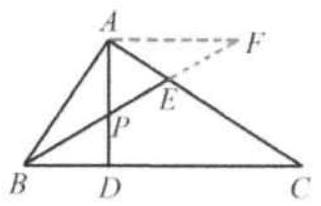
\includegraphics[width=\textwidth]{images/108.jpg}

Thus \(\frac{B D}{B C}=\frac{B D}{B D+D C}=\frac{1}{1+k^{2}}\).\\
Therefore \(\frac{A E}{E C}=\frac{1}{1+k^{2}}\).



\end{document}
